\begin{center}
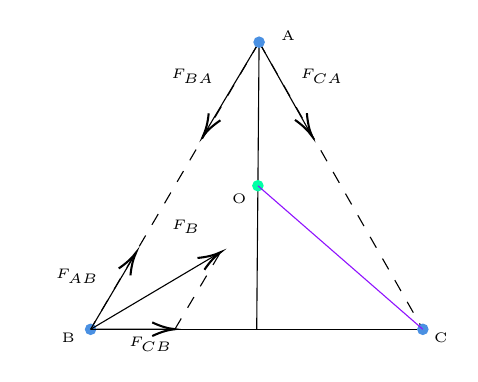
\begin{tikzpicture}[x=0.75pt,y=0.75pt,yscale=-1,xscale=1]
%uncomment if require: \path (0,300); %set diagram left start at 0, and has height of 300

%Straight Lines [id:da7411767697224816] 
\draw    (100,102) ;
%Straight Lines [id:da35334013949437937] 
\draw    (130.05,191.39) -- (290.12,191.39) ;
%Straight Lines [id:da8337888464734036] 
\draw    (211.23,53.05) -- (210.08,191.39) ;
%Straight Lines [id:da37892752623854364] 
\draw    (211.23,53.05) -- (185.19,96.68) ;
\draw [shift={(184.17,98.4)}, rotate = 300.82] [color={rgb, 255:red, 0; green, 0; blue, 0 }  ][line width=0.75]    (10.93,-3.29) .. controls (6.95,-1.4) and (3.31,-0.3) .. (0,0) .. controls (3.31,0.3) and (6.95,1.4) .. (10.93,3.29)   ;
%Straight Lines [id:da23461063513640812] 
\draw  [dash pattern={on 4.5pt off 4.5pt}]  (211.23,53.05) -- (130.05,191.39) ;
%Straight Lines [id:da4163775253760995] 
\draw  [dash pattern={on 4.5pt off 4.5pt}]  (211.23,53.05) -- (290.12,191.39) ;
%Straight Lines [id:da14314395431520932] 
\draw    (211.23,53.05) -- (235.78,96.66) ;
\draw [shift={(236.76,98.4)}, rotate = 240.62] [color={rgb, 255:red, 0; green, 0; blue, 0 }  ][line width=0.75]    (10.93,-3.29) .. controls (6.95,-1.4) and (3.31,-0.3) .. (0,0) .. controls (3.31,0.3) and (6.95,1.4) .. (10.93,3.29)   ;
%Shape: Circle [id:dp27435800391771203] 
\draw  [color={rgb, 255:red, 74; green, 144; blue, 226 }  ,draw opacity=1 ][fill={rgb, 255:red, 74; green, 144; blue, 226 }  ,fill opacity=1 ] (213.73,53.05) .. controls (213.73,51.67) and (212.61,50.55) .. (211.23,50.55) .. controls (209.85,50.55) and (208.73,51.67) .. (208.73,53.05) .. controls (208.73,54.43) and (209.85,55.55) .. (211.23,55.55) .. controls (212.61,55.55) and (213.73,54.43) .. (213.73,53.05) -- cycle ;
%Shape: Circle [id:dp355067680258665] 
\draw  [color={rgb, 255:red, 74; green, 144; blue, 226 }  ,draw opacity=1 ][fill={rgb, 255:red, 74; green, 144; blue, 226 }  ,fill opacity=1 ] (132.55,191.39) .. controls (132.55,190.01) and (131.43,188.89) .. (130.05,188.89) .. controls (128.67,188.89) and (127.55,190.01) .. (127.55,191.39) .. controls (127.55,192.77) and (128.67,193.89) .. (130.05,193.89) .. controls (131.43,193.89) and (132.55,192.77) .. (132.55,191.39) -- cycle ;
%Shape: Circle [id:dp8731378911211072] 
\draw  [color={rgb, 255:red, 74; green, 144; blue, 226 }  ,draw opacity=1 ][fill={rgb, 255:red, 74; green, 144; blue, 226 }  ,fill opacity=1 ] (292.62,191.39) .. controls (292.62,190.01) and (291.5,188.89) .. (290.12,188.89) .. controls (288.74,188.89) and (287.62,190.01) .. (287.62,191.39) .. controls (287.62,192.77) and (288.74,193.89) .. (290.12,193.89) .. controls (291.5,193.89) and (292.62,192.77) .. (292.62,191.39) -- cycle ;
%Shape: Circle [id:dp08553461642771443] 
\draw  [color={rgb, 255:red, 0; green, 255; blue, 165 }  ,draw opacity=1 ][fill={rgb, 255:red, 0; green, 255; blue, 165 }  ,fill opacity=1 ] (213.15,122.22) .. controls (213.15,120.84) and (212.04,119.72) .. (210.65,119.72) .. controls (209.27,119.72) and (208.15,120.84) .. (208.15,122.22) .. controls (208.15,123.6) and (209.27,124.72) .. (210.65,124.72) .. controls (212.04,124.72) and (213.15,123.6) .. (213.15,122.22) -- cycle ;
%Straight Lines [id:da7509716289501367] 
\draw [color={rgb, 255:red, 144; green, 19; blue, 254 }  ,draw opacity=1 ]   (210.65,122.22) -- (290.12,191.39) ;
%Straight Lines [id:da6715627766530636] 
\draw    (130.05,191.39) -- (168.67,191.34) ;
\draw [shift={(170.67,191.33)}, rotate = 179.92] [color={rgb, 255:red, 0; green, 0; blue, 0 }  ][line width=0.75]    (10.93,-3.29) .. controls (6.95,-1.4) and (3.31,-0.3) .. (0,0) .. controls (3.31,0.3) and (6.95,1.4) .. (10.93,3.29)   ;
%Straight Lines [id:da8234752419975047] 
\draw    (130.05,191.39) -- (150.98,156.05) ;
\draw [shift={(152,154.33)}, rotate = 120.64] [color={rgb, 255:red, 0; green, 0; blue, 0 }  ][line width=0.75]    (10.93,-3.29) .. controls (6.95,-1.4) and (3.31,-0.3) .. (0,0) .. controls (3.31,0.3) and (6.95,1.4) .. (10.93,3.29)   ;
%Straight Lines [id:da371469419005255] 
\draw  [dash pattern={on 4.5pt off 4.5pt}]  (170.67,191.33) -- (192.62,154.27) ;
%Straight Lines [id:da13561111516549063] 
\draw    (130.05,191.39) -- (190.9,155.29) ;
\draw [shift={(192.62,154.27)}, rotate = 149.32] [color={rgb, 255:red, 0; green, 0; blue, 0 }  ][line width=0.75]    (10.93,-3.29) .. controls (6.95,-1.4) and (3.31,-0.3) .. (0,0) .. controls (3.31,0.3) and (6.95,1.4) .. (10.93,3.29)   ;

% Text Node
\draw (220.67,46.33) node [anchor=north west][inner sep=0.75pt]  [font=\tiny] [align=left] {A};
% Text Node
\draw (115,192) node [anchor=north west][inner sep=0.75pt]  [font=\tiny] [align=left] {B};
% Text Node
\draw (294.33,192) node [anchor=north west][inner sep=0.75pt]  [font=\tiny] [align=left] {C};
% Text Node
\draw (197,125) node [anchor=north west][inner sep=0.75pt]  [font=\tiny] [align=left] {O};
% Text Node
\draw (167.67,64.67) node [anchor=north west][inner sep=0.75pt]  [font=\tiny] [align=left] {$\displaystyle F_{BA}$};
% Text Node
\draw (230,64.67) node [anchor=north west][inner sep=0.75pt]  [font=\tiny] [align=left] {$\displaystyle F_{CA}$};
% Text Node
\draw (112,161) node [anchor=north west][inner sep=0.75pt]  [font=\tiny] [align=left] {$\displaystyle F_{AB}$};
% Text Node
\draw (147.33,194) node [anchor=north west][inner sep=0.75pt]  [font=\tiny] [align=left] {$\displaystyle F_{CB}$};
% Text Node
\draw (168,137.33) node [anchor=north west][inner sep=0.75pt]  [font=\tiny] [align=left] {$\displaystyle F_{B}$};
\end{tikzpicture}

\end{center}